\documentclass[report.tex]{subfiles}
\begin{document}
\section{Definitions}
Before describing the AES encryption, some key definitions need to be mentioned

\subsection{Addition}\label{sec:addition}
In the AES standard, addition is performed bitwise with the XOR operator. No regard is taken to carry bits. Consequently, subtraction is identical to addition.

\subsection{Multiplication}\label{sec:multiplication}
In the AES standard, multiplication is performed by using the multiplication of polynomial modulo an irreducible polynomial of degree 8, GF$\left(2^{8}\right)$ 
\begin{comment}
	\cite[Sec.~4.2]{AES Standard}
\end{comment}
where GF is short for Rijndael's finite field or Galois field 
\begin{comment}
	\cite{GF} page = http://en.wikipedia.org/wiki/Rijndael_Galois_field#Rijndael.27s_finite_field, date=2011-11-14
\end{comment}
. this means that multiplication is performed by using addition defined in \ref{sec:addition} between the resulting terms and then dividing the result with a given polynomial.

The polynomia used in the AES standard is
\begin{equation} \label{eq:multiplication polynomial}
	{x^{8} + x^{4} + x^{3} + x + 1} = 11B_{16} = 283_{10}.
\end{equation}


\subsection{Cipher key}
A cipher key is a secret "passphrase" shared between the encryption and decryption side. It is the single most important part of a crypto; once the cipher key is known, all data encrypted with that key can be decrypted.

\subsection{Key length} \label{sec:key length}
The key length determine how many bits are used to encrypt input data. The AES standard defines 3 key lengths: AES-128, AES-192 and AES-256.

The key length is commonly used to denote the strength of the AES encryption.

\subsection{Block}
Data and keys are organized in 4xN matrices called blocks (Figure \ref{fig:block definition}). Each element defines 1 byte and each column is 1 word (32 bits). A block is read one column at a time and each column from the top down.

\begin{figure}[h]
%\setlength{\unitlength}{1.0cm}
\centering
		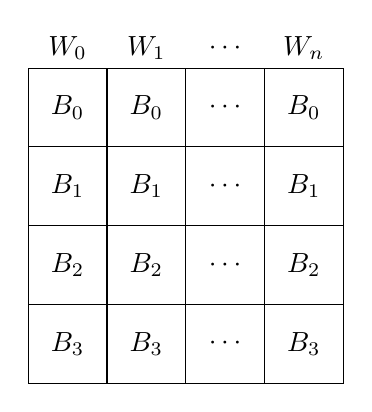
\begin{tikzpicture}
			\foreach \y/\wordtext in {0/W_{\y},1/W_{\y},2/\cdots,3/W_{n}}
			{
				
				\foreach \x/\bytetext in {0/B_{\y},1/B_{\y},2/\cdots,3/B_{\y}}
				{
					\node[draw, shape=rectangle, minimum height=1cm, minimum width=1cm, inner sep=0] () at (\x,3 - \y){$\bytetext$};	
				}
				\node () at (\y, 3.75){$\wordtext$};
			}
		\end{tikzpicture}
	\caption{Block definition}
	\label{fig:block definition}
\end{figure}

Input, state and output data is always in 4x4 blocks (128 bits) while cipher keys can have varying lengths (see section \ref{sec:key length}).

\subsection{Round}
Encryption of data works by manipulating the input data in an iterative process where each iteration is called a round. The number of rounds needed is determined by the cipher key length.

To calculate the number of rounds needed for a specific key length, (\ref{eq:round length}) can be used
\begin{equation}\label{eq:round length}
	N_r = 6 + \frac{A_{l}}{W_{l}}
\end{equation}
where $A_l$ and $W_l$ denotes key length (128, 192 or 256 bit) and word length (32 bit) respectively.

\subsection{Round key}
For each round in the encryption process a different round key is used. In total there are $N_r+1$ round keys. More on this in section \ref{sec:theory}

\subsection{State block or state array}
Data to be encrypted (input data) is copied to a state block. During intermediate encryption rounds, data is manipulated on the state block. After the final round the state block is copied to the output block.% See figure \ref{fig:state array}.

\begin{figure}[h]
\centering
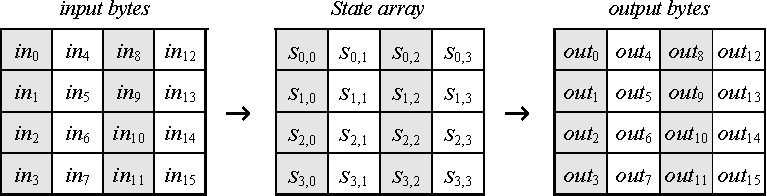
\includegraphics[width=\linewidth]{state_array}
\caption{State array input and output. Source: fips}
\label{fig:state array}
\end{figure}

\end{document}